\usetikzlibrary{positioning,matrix,fit}
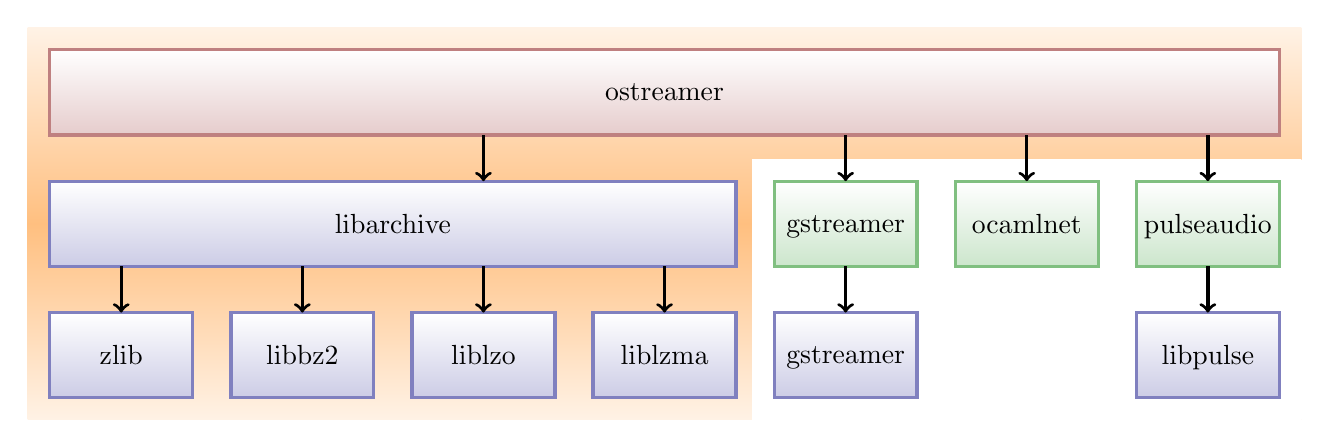
\begin{tikzpicture}[
  redblock/.style={
    rectangle,
    very thick,
    draw=red!50!black!50,
    top color=white,
    bottom color=red!50!black!20,
    inner sep=0em
  },
 blueblock/.style={
    rectangle,
    very thick,
    draw=blue!50!black!50,
    top color=white,
    bottom color=blue!50!black!20,
    inner sep=0em
  },
 greenblock/.style={
    rectangle,
    very thick,
    draw=green!50!black!50,
    top color=white,
    bottom color=green!50!black!20,
    inner sep=0em,
  },
  highlight/.style={
    rectangle,
    top color=orange!10,
    bottom color=orange!10,
    % middle color goes last
    middle color=orange!50,
    inner sep=0.8em,
  },
  nohighlight/.style={
    rectangle,
    top color=white,
    bottom color=white,
    inner sep=0.8em,
  },
  testblock/.style={
    draw,
    inner sep=0mm
  }]
      \matrix (table) [%
        minimum width = 18mm,
        %draw,
        matrix of nodes,
        nodes in empty cells,
        row  sep=6mm,column sep=5mm
        ]{
  & & & & & & \\
  & & & & & & \\
  & & & & & & \\
  & & & & & & \\
  & & & & & & \\
  & & & & & & \\
 };
  % highlight
  \node [highlight, fit=(table-1-1)(table-6-7)] {};
  \node [nohighlight, fit=(table-3-5)(table-6-7)] {};
  % level 1
  \node [redblock,fit=(table-1-1)(table-2-7),label={center:ostreamer}] {};
  % level 2
  \node [blueblock,fit=(table-3-1)(table-4-4),label={center:libarchive}] {};
  \node [greenblock,fit=(table-3-5)(table-4-5),label={[text depth=0]center:gstreamer}] {};
  \node [greenblock,fit=(table-3-6)(table-4-6),label={center:ocamlnet}] {};
  \node [greenblock,fit=(table-3-7)(table-4-7),label={[text depth=0]center:pulseaudio}] {};
 % level 3
  \node [blueblock,fit=(table-5-1)(table-6-1),label={center:zlib}] {};
  \node [blueblock,fit=(table-5-2)(table-6-2),label={center:libbz2}] {};
  \node [blueblock,fit=(table-5-3)(table-6-3),label={center:liblzo}] {};
  \node [blueblock,fit=(table-5-4)(table-6-4),label={center:liblzma}] {};
  \node [blueblock,fit=(table-5-5)(table-6-5),label={[text depth=0]center:gstreamer}] {};
  \node [blueblock,fit=(table-5-7)(table-6-7),label={[text depth=0]center:libpulse}] {};
  \begin{scope}
  % level 2
  \draw[->,very thick] (table-2-3) -- (table-3-3);
  \draw[->,very thick] (table-2-5) -- (table-3-5);
  \draw[->,very thick] (table-2-6) -- (table-3-6);
  \draw[->,very thick] (table-2-7) -- (table-3-7);
  % level 3
  \draw[->,very thick] (table-4-1) -- (table-5-1);
  \draw[->,very thick] (table-4-2) -- (table-5-2);
  \draw[->,very thick] (table-4-3) -- (table-5-3);
  \draw[->,very thick] (table-4-4) -- (table-5-4);
  \draw[->,very thick] (table-4-5) -- (table-5-5);
  \draw[->,very thick] (table-4-7) -- (table-5-7);
  \end{scope}
\end{tikzpicture}
% http://tex.stackexchange.com/questions/94343/matrix-of-nodes-over-multiple-columns-in-tikz